\documentclass[acmlarge]{acmart}
\usepackage{subfig}
\usepackage{booktabs} % For formal tables
\usepackage[ruled]{algorithm2e} % For algorithms
\renewcommand{\algorithmcfname}{ALGORITHM}
\SetAlFnt{\small}
\SetAlCapFnt{\small}
\SetAlCapNameFnt{\small}
\SetAlCapHSkip{0pt}
\IncMargin{-\parindent}

% Metadata Information
%\acmJournal{PACMHCI}
%\acmVolume{9}
%\acmNumber{4}
%\acmArticle{39}
%\acmYear{2010}
%\acmMonth{3}
%\acmArticleSeq{11}

%\acmBadgeR[http://ctuning.org/ae/ppopp2016.html]{ae-logo}
%\acmBadgeL[http://ctuning.org/ae/ppopp2016.html]{ae-logo}


% Copyright
%\setcopyright{acmcopyright}
%\setcopyright{acmlicensed}
%\setcopyright{rightsretained}
%\setcopyright{usgov}
%\setcopyright{usgovmixed}
%\setcopyright{cagov}
%\setcopyright{cagovmixed}

% DOI
%\acmDOI{0000001.0000001}

% Paper history
%\received{February 2007}
%\received{March 2009}
%\received[accepted]{June 2009}


% Document starts
\begin{document}
% Title portion
\title{On the Internal Evaluation of Unsupervised Outlier Detection} 
%\titlenote{We can add a note to the title}

\author{Henrique O. Marques}
%\authornote{This is the corresponding author}
%\orcid{1234-5678-9012-3456}
\affiliation{%
  \institution{University of S\~ao Paulo}
  \city{S\~ao Carlos}
  %\state{SP}
  \country{Brazil}}
\email{hom@icmc.usp.br}
\author{Ricardo J. G. B. Campello}
\affiliation{%
  \institution{James Cook University}
  \city{Townsville}
  \country{Australia}
}
\email{ricardo.campello@jcu.edu.au}
\author{Arthur Zimek} 
\affiliation{%
 \institution{University of Southern Denmark}
 %\streetaddress{Rono-Hills}
 \city{Odense} 
 %\state{Arunachal Pradesh}
 \country{Denmark}}
\email{zimek@imada.sdu.dk}
\author{J{\"o}rg Sander}
\affiliation{%
  \institution{University of Alberta}
  %\streetaddress{30 Shuangqing Rd}
  \city{Edmonton} 
  %\state{Beijing Shi}
  \country{Canada}
}
\email{jsander@ualberta.ca}



\begin{abstract}

\end{abstract}


%
% The code below should be generated by the tool at
% http://dl.acm.org/ccs.cfm
% Please copy and paste the code instead of the example below. 
%
\begin{CCSXML}
<ccs2012>
 <concept>
  <concept_id>10010520.10010553.10010562</concept_id>
  <concept_desc>Computer systems organization~Embedded systems</concept_desc>
  <concept_significance>500</concept_significance>
 </concept>
 <concept>
  <concept_id>10010520.10010575.10010755</concept_id>
  <concept_desc>Computer systems organization~Redundancy</concept_desc>
  <concept_significance>300</concept_significance>
 </concept>
 <concept>
  <concept_id>10010520.10010553.10010554</concept_id>
  <concept_desc>Computer systems organization~Robotics</concept_desc>
  <concept_significance>100</concept_significance>
 </concept>
 <concept>
  <concept_id>10003033.10003083.10003095</concept_id>
  <concept_desc>Networks~Network reliability</concept_desc>
  <concept_significance>100</concept_significance>
 </concept>
</ccs2012>  
\end{CCSXML}

\ccsdesc[500]{Computer systems organization~Embedded systems}
\ccsdesc[300]{Computer systems organization~Redundancy}
\ccsdesc{Computer systems organization~Robotics}
\ccsdesc[100]{Networks~Network reliability}

%
% End generated code
%


\keywords{Wireless sensor networks, media access control,
multi-channel, radio interference, time synchronization}

% DO NOT use this command unless you want to change
% the default behavior
% \authorsaddresses{Authors' addresses: G.~Zhou, Computer Science
%   Department, College of William and Mary, 104 Jameson Rd,
%   Williamsburg, PA 23185, US, \path{gzhou@wm.edu}; V.~B\'eranger,
%   Inria Paris-Rocquencourt, Rocquencourt, France; A.~Patel, Rajiv
%   Gandhi University, Rono-Hills, Doimukh, Arunachal Pradesh, India;
%   H.~Chan, Tsinghua University, 30 Shuangqing Rd, Haidian Qu, Beijing
%   Shi, China; T.~Yan, Eaton Innovation Center, Prague, Czech Republic;
%   T.~He, C.~Huang, J.~A.~Stankovic University of Virginia, School of
%   Engineering Charlottesville, VA 22903, USA; T. F. Abdelzaher,
%   (Current address) NASA Ames Research Center, Moffett Field,
%   California 94035.}

\maketitle

% The default list of authors is too long for headers.
\renewcommand{\shortauthors}{H. O. Marques et al.}

%!TEX root = sample-acmlarge.tex

\section{Introduction}
%!TEX root = ../sample-acmlarge.tex

\subsection{Related Work}
\subsection{Contributions}
\subsection{Outline of the Article}


\newpage
\section{IREOS Revisited}
%!TEX root = ../sample-acmlarge.tex
Let $\mathbf{X} = \{\mathbf{x}_1, \cdots, \mathbf{x}_N \}$ be an unlabeled data set containing $N$ $d$-dimensional feature vectors, $\mathbf{x}_i$, and assume that one or more unsupervised outlier detection algorithms will produce, for this data set, candidate outliers solutions, which one wants to evaluate in the absence of labels. Solutions produced by unsupervised outlier detection algorithms can be given in different formats. The most common format is given as a set $\mathbf{y} = \{ y_1, \cdots, y_N \}$, $y_i \in \mathbb{R}^+$, where $y_i$ represents the outlier score associated with the observation $\mathbf{x}_i$, that reflects the degree of outlierness of $\mathbf{x}_i$. Such solutions allow that the observations $\mathbf{x}_i$ be sorted and ranked according to their degree of outlierness $y_i$. When the number of outliers $n$ is known, one can establish a threshold in the ranking in order to select a subset $\mathbf{S} \subset \mathbf{X}$, $|\mathbf{S}| = n$, containing the top-$n$ observations that are labeled as outliers. Given a collection of candidate solutions $\mathbf{S}$, usually called of top-$n$ (binary) outlier detection solution, IREOS \cite{marques2015} is able to independently and quantitatively measure the quality of each individual candidate solution in the absence of labels.

The criteria used by IREOS is based on the common intuition that an outlier is an observation that is to some extent farther off and can therefore be more easily separated (discriminated) from other observations than an inlier. In order to quantify how easily an observation can be separated from the other observations, IREOS uses a maximum margin classifier \cite{bishop2006,hastie2013} to assess the separability of individual observations, using the distance from the observation to the decision boundary as the base of the separability measure used in the evaluation. However, the separation of certain observations (such as those within a cluster) implies in the use of nonlinear maximum margin classifiers, such as Support Vector Machine (SVM) or Kernel Logistic Regression (KLR) \cite{bishop2006,hastie2013}, as these observations require nonlinear decision boundary to be separated. These classifiers use a kernel function, such as the radial basis kernel \cite{scholkopf2001}, to transform the original (possibly non-linearly separable) problem into a linearly separable one. The use of a kernel function demands the configuration of the kernel parameter $\gamma$. According to the discussion in \citep{marques2015}, the choice of a single parameter value is not necessary for this problem, instead, a range of value of $\gamma$ from 0 up to a maximum value $\gamma_{max}$ (for which all the observations labeled as outliers can be individually discriminated from all the others by using a kernel-based classifier) is chosen and the \textit{area under the curve} (AUC) formed by the overall separability of an observation $\mathbf{x}_i$ over the interval of $\gamma$ values (Fig. \ref{fig:ind_avg_curv}) is taken,

\begin{equation}
\int_{\gamma = 0}^{\gamma_{max}} p(\mathbf{x}_i, \gamma)
\end{equation}
where $p(\mathbf{x}_i, \gamma)$ quantifies in a normalized interval how far each observation $\mathbf{x}_i$ is from the decision boundary.

In order to evaluate the quality of a given solution $\mathbf{S}$, the average curve of separability for those observations in $\mathbf{S}$ is taken, 

\begin{equation}
\int_{\gamma = 0}^{\gamma_{max}} \bar{p}(\gamma) = \int_{\gamma = 0}^{\gamma_{max}} \frac{1}{n} \sum_{\mathbf{x}_i \in \mathbf{S}} p(\mathbf{x}_i, \gamma)
\label{eq:ireos:avg_curve}
\end{equation}

As in practice classifiers need to be trained to compute $\bar{p}(\gamma)$ for each $\gamma$, the interval $[0, \gamma_{max}]$ is discretized into a finite number of values for $\gamma$, from $\gamma_1 = 0$ to $\gamma_{n_\gamma} = \gamma_{max}$, and the index can thus be computed (within $[0, 1]$) as:

\begin{equation}
I(\mathbf{S}) = \frac{1}{n_{\gamma}} \sum_{l = 1}^{n_{\gamma}} \left( \frac{1}{n} \sum_{\mathbf{x}_i \in \mathbf{S}} p(\mathbf{x}_i, \gamma_l) \right)
\label{eq:original_ireos}
\end{equation}

\subsection{Modeling clumps}

Clumps, or particles, are subsets of observations lying in the same region of the data space, relatively close to each other than they are from other observations, but too small to be deemed a cluster. In order to modeling the presence of possible clumps, IREOS proposes the use of soft margin classifiers with individual penalties for each observation \cite{osuna1997}. These classifiers allow the misclassification of observations at the price of a penalty term $P_t$ (the cost of the misclassification can be different for each observation) that is incorporated into the original objective of margin maximization. Such a term is typically in the form
\begin{equation}
P_t = \sum_{i = 1}^{N}C(\mathbf{x}_i)\xi(\mathbf{x}_i), 
\end{equation}
where $\xi(\mathbf{x}_i)$ stands for the individual penalty component associated with observation $\mathbf{x}_i$. The farther an observation $\mathbf{x}_i$ is from the margin boundary on the wrong side, the greater the value of $\xi(\mathbf{x}_i)$. $C(\mathbf{x}_i)$ controls the cost of penalties of the observations $\mathbf{x}_i$, where the full cost $C$ is assigned to the observations labeled as inliers ($C(\mathbf{x}_i) = C$) yet only a fraction $\beta \in [0, 1]$ of $C$ to the observations labeled as outliers ($C(\mathbf{x}_i) = \beta \cdot C$). The setting of $\beta$ controls the effect that the labeling of the other observations will have when assessed the separability of a particular observation. For $\beta = 1$, the method reduces to the ordinary case where observations are treated equally no matter their labels. In the other extreme, $\beta = 0$, observations labeled as outliers can be misclassified for free (notice that, when evaluating the separability of a specific observation, this is equivalent to removing all other observations labeled as outliers from the data set).

The fraction of the penalty ($\beta$) is set from an optional control parameter introduced by IREOS, the maximum clump size ($m_{cl}$), that allow the users adjust their expectations about clump sizes. The optional control parameter is set as $\beta = \frac{1}{m_{cl}}$. The control parameter is optional because by setting $m_{cl} = 1$, the method reduces to the particular case where clumps are not modeled and the same, full penalty cost is assigned to all observations. By setting $\beta = \frac{1}{m_{cl}}$, one needs $m_{cl}$ observations (a full clump) labeled as outliers to get the same impact as a single inlier. Notice that except when $m_{cl} = 1$, the separability of each observation in the general case depends on the labels of the other observations.

%The maximum clump size, $m_{cl}$, is a mechanism that allows different users in varied application scenarios to explicitly express what they judge ``too small'' to be interpreted as a cluster.
%The possible presence of clumps in the data set induces IREOS to provide the users with an optional control mechanism to adjust their expectations about clump sizes. 

\newpage
\section{Internal Evaluation of Unsupervised Outlier Detection}
%!TEX root = ../sample-acmlarge.tex
Although the IREOS index was the first, and so far the only, internal index devoted to bridging the gap related to the internal evaluation of outlier detection results \cite{zimek2013,marques2015}, it has the main limitation of restricting to directly evaluate only top-$n$ (binary) outlier detection results $\mathbf{S}$. Without previously know the number of outliers in the dataset $n$, it is not possible to evaluate a solution given as outlier scoring $\mathbf{y}$. In this section, we devise means to extend IREOS to evaluate a collection of candidate solutions $\mathbf{y}$ in the absence of labels and independent of a choice of $n$.

\subsection{Internal Evaluation of Top-n Outlier Detection Results}
Since the observations $\mathbf{x}_i$ are sorted and ranked according to their degree of outlierness $y_i$ and the threshold in the ranking is established, the top-$n$ observations can be labeled as outliers. Even though it is clear that the best solution must rank all outliers before all inliers and the worst solution must rank all inliers before all outliers, there are $n!$ different possible best top-$n$ solutions equally well rated. However, the truly best outlier solution should rank more obvious or clear outliers before less obvious outliers before those that could be outliers or inliers and so on. This issue was already discussed and addressed by \cite{schubert2012} in the context of the external evaluation of outlier detection, once that the main external measures (\textit{e.g.} ROC AUC and $prec@n$) cannot make such distinction. As well as these external measures, IREOS cannot differentiate the quality of these $n!$ different possible best solutions.

We start the IREOS extension addressing the problem discussed above, in order to make possible distinguish the quality of the ranks among the top-$n$ observations, we introduced weights in the Equation \ref{eq:ireos:avg_curve} where the average curve of separability is defined, so that the average curve of separability becomes a weighted average curve of separability,
\begin{equation}
\int_{\gamma = 0}^{\gamma_{max}} \bar{p}(\gamma) = \int_{\gamma = 0}^{\gamma_{max}} \frac{1}{\sum_{\mathbf{x}_i \in \mathbf{S}} w_i} \sum_{\mathbf{x}_i \in \mathbf{S}} p(\mathbf{x}_i, \gamma) w_i
\label{eq:w_avg_sep}
\end{equation}
where $w_i$ stands for the weight associated with the observation $\mathbf{x}_i$. The use of weights in the outlier evaluation was already discussed by \cite{schubert2012}, the authors argue that the choice of a score-based approach is a good option for several reasons, but when comparing different methods that have different scales, some kind of normalization is unavoidable. Following the authors' recommendation, we use the outlier scoring normalization framework proposed by \cite{kriegel2011}, as this framework proposes a variety of normalization methods based on statistics and distribution fitting that can accommodate several outlier detection algorithms. Thus, the normalized outlier scores $w_i$ are used as the weights associated to observations $\mathbf{x}_i$.

By introducing the score-based weights we expected that in the truly best solution, the outlier scores and the separabilities of the more obvious outliers to be higher, whereas in a false best solution, while the outlier scores of the less obvious outliers are expected to be higher, their separabilities are expected to be lower. Therefore, when combined the higher outlier scores with the higher separabilities and the lower outlier scores with lower separabilities of the truly best solution, it will produce a larger AUC, when compared with AUC produced by a false best solution that combines higher outlier scores with lower separabilities and lower outlier scores with higher separabilities. An illustrative example is provided in Fig. \ref{fig:ilustration}. In Fig. \ref{fig:data} three observations are labeled as outliers in a hypothetical top-$n$ outlier detection solution, a more obvious outlier (blue square), a less obvious outlier (green circle) and a not obvious outlier (red diamond). Their separabilities are individually assessed in the Fig. \ref{fig:ind_avg_curv}. In Fig. \ref{fig:avg_sep_curv} two variations of this top-$n$ outlier solution are presented, differing in the outlier scores ranking. The named truly best solution ranks the more obvious outlier (outlier score 1) before the less obvious outlier (outlier score 0.75) before the not obvious outlier (0.51), the reverse ranking of the false best solution that ranks the not obvious outlier (outlier score 1) before the less obvious outlier (outlier score 0.75) before the more obvious outlier (0.51). These two different solutions would be equally well rated for the main external measures AUC ROC and $prec@n$ as well as IREOS before the proposed extension. However, using the proposed weighted average curve of separability the index can properly evaluate the solution, as expected the truly best solution has a larger AUC than the false best solution, so the quality of the truly best solution is higher than the false best solution.

\begin{figure}[ht!]
\center
\subfloat[Illustrative dataset]{\label{fig:data} 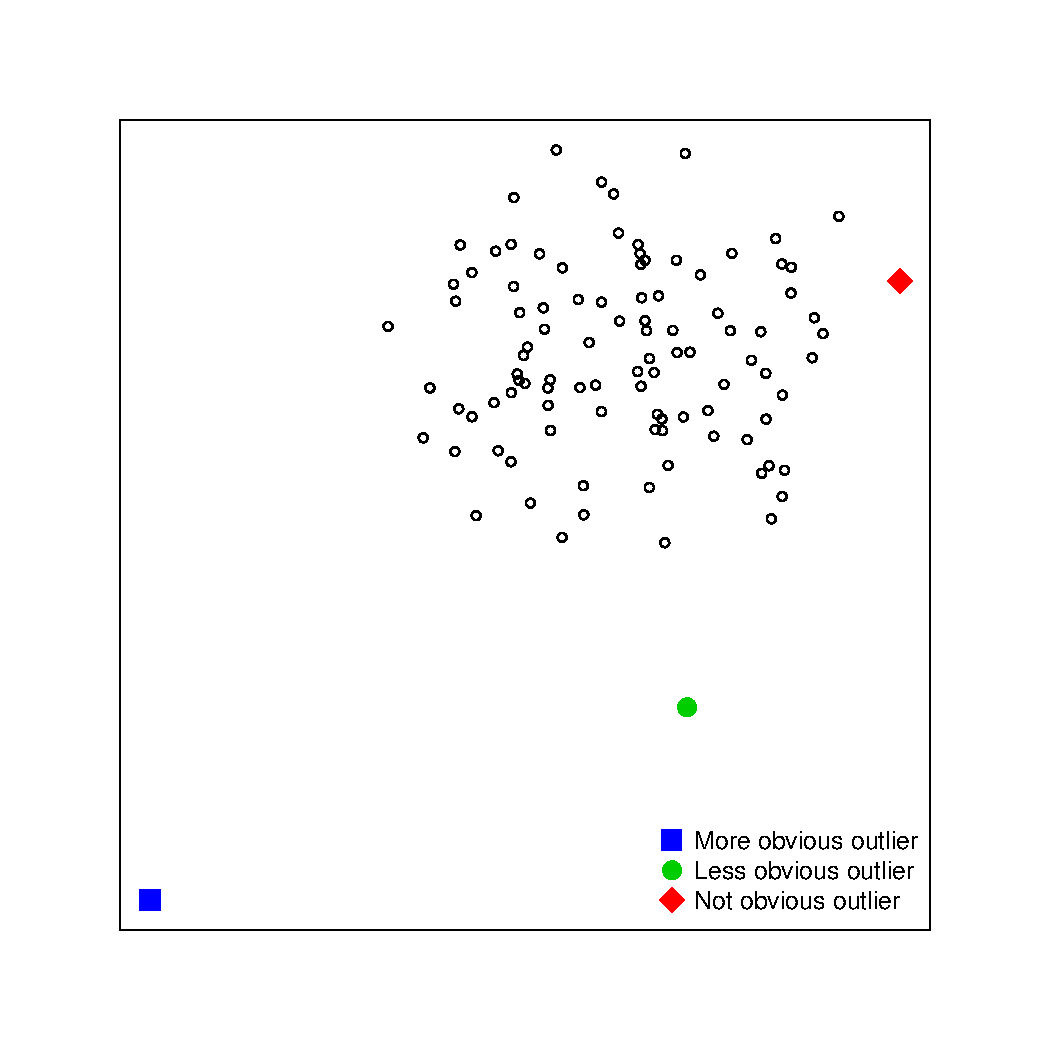
\includegraphics[width=4.7cm]{figs/data.pdf}}
\qquad
\subfloat[Individual separability curves]{\label{fig:ind_avg_curv} 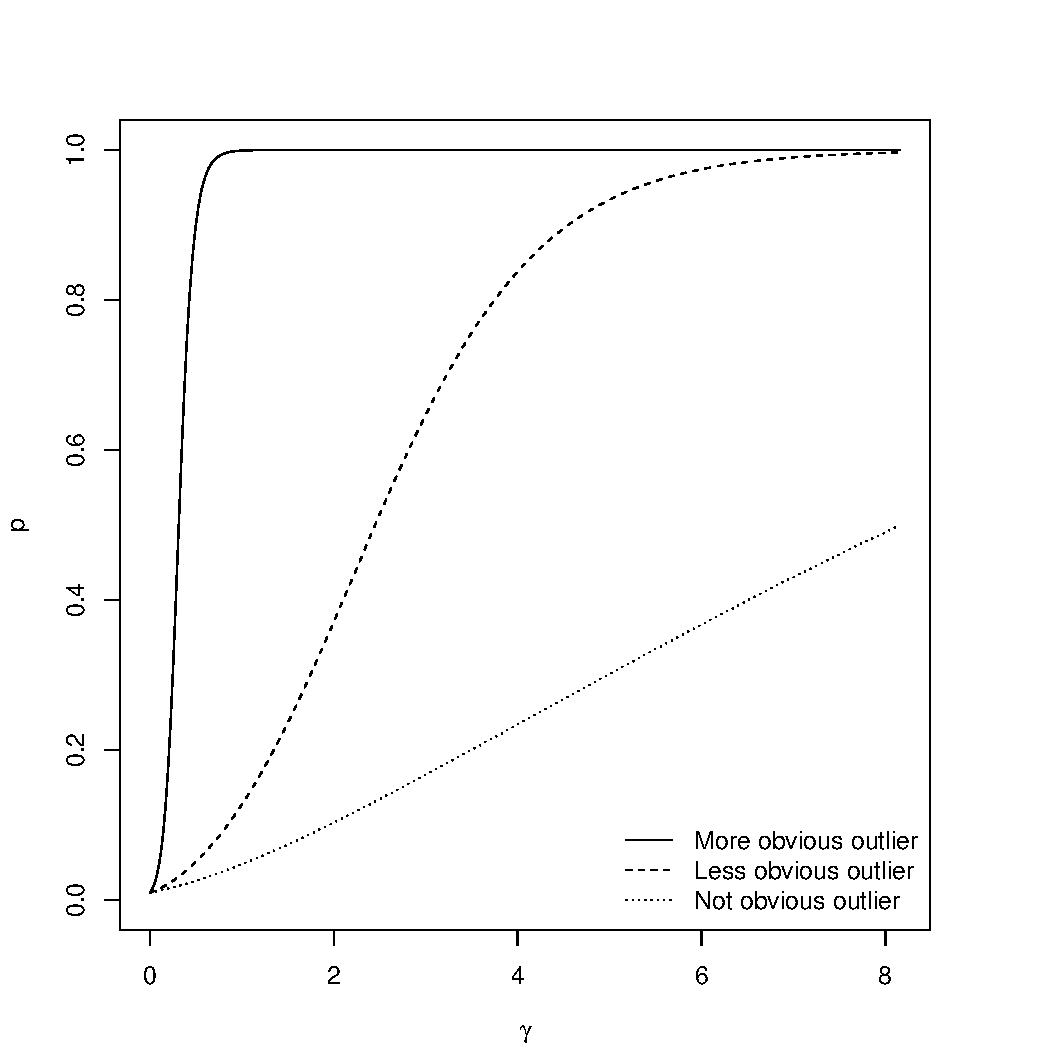
\includegraphics[width=4.7cm]{figs/sep_curves.pdf}}
\qquad
\subfloat[Weighted average curve of separability]{\label{fig:avg_sep_curv} 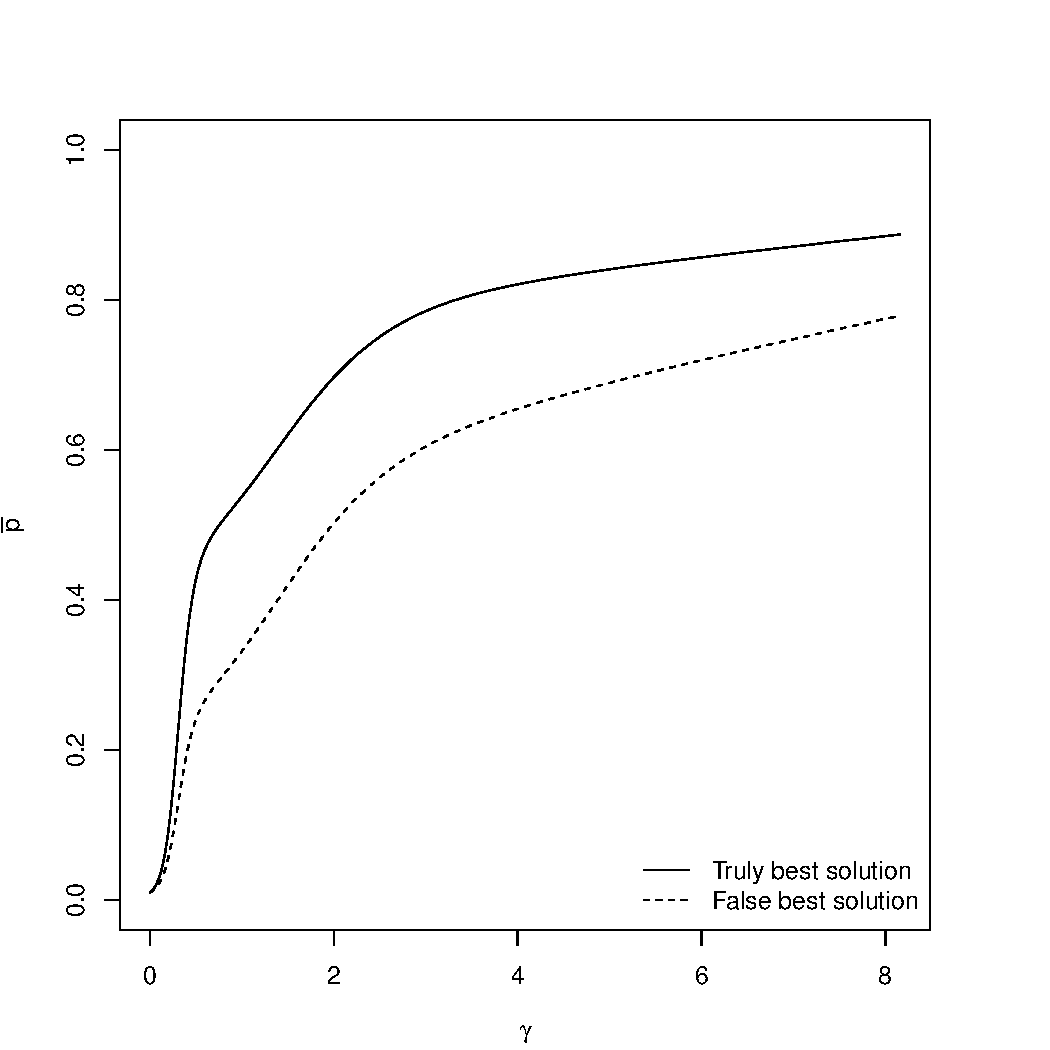
\includegraphics[width=4.7cm]{figs/avg_sep_curves.pdf}}
\caption{Illustrative example of a top-$n$ outlier solution: In \ref{fig:data} the top three observations are labeled as outliers; Their separabilities are individually assessed in \ref{fig:ind_avg_curv}; The outlier scorings of the two different top-$n$ solutions are evaluated in \ref{fig:avg_sep_curv}, the outlier scores of the more obvious outlier, the less obvious outlier and not obvious outliers are respectively 1, 0.75, 0.51 for the truly best solution and 0.51, 0.75, 1 for the false best solution}
\label{fig:ilustration}
\end{figure}

The extension proposed here is computed similarly to the original index presented in the Equation \ref{eq:original_ireos}. However, instead of use the average curve of separability (Equation \ref{eq:ireos:avg_curve}) we use the weighted average curve of separability (Equation \ref{eq:w_avg_sep}):
\begin{equation}
I(\mathbf{S}) = \frac{1}{n_{\gamma}} \sum_{l = 1}^{n_{\gamma}} \left( \frac{1}{\sum_{\mathbf{x}_i \in \mathbf{S}} w_i} \sum_{\mathbf{x}_i \in \mathbf{S}} p(\mathbf{x}_i, \gamma_l) w_i \right)
\label{eq:ext_ireos}
\end{equation}

Note that giving the same scores for all observations labeled as outliers the index of the Equation \ref{eq:ext_ireos} will be reduced to the original index of the Equation \ref{eq:original_ireos}, where the followed assumption is that all the observations labeled are equally outliers.

\subsection{Internal Evaluation of Scoring Outlier Detection Results}
From the first extension is easy to note that such index could be trivially extended in order to evaluate the whole outlier scorings. As we intend to evaluate the solution without make the assumption that the number of outliers in the dataset is known, we take into account the whole dataset $\mathbf{X}$ in the evaluation, instead of the only top-$n$ outlier observations present in $\mathbf{S}$:
\begin{equation}
I(\mathbf{S}) = \frac{1}{n_{\gamma}} \sum_{l = 1}^{n_{\gamma}} \left( \frac{1}{\sum_{\mathbf{x}_i \in \mathbf{X}} w_i} \sum_{\mathbf{x}_i \in \mathbf{X}} p(\mathbf{x}_i, \gamma_l) w_i \right)
\end{equation}

Note that with the scoring normalization proposed by \cite{kriegel2011}, the outlier scores of the inliers is expected to be close to 0\footnote{with the proposed normalization by \cite{kriegel2011}, it will often be in fact 0}, therefore, they will affect very little in the quality of the solution.  Moreover, the exchange between observations with similar scores will be slightly penalized (\textit{e. g.} the exchange between clear outliers, or between clear inliers), while the exchange between observations with a great contrast in the outlier scorings will be highly penalized (\textit{e. g.} the exchange between a clear outlier and a clear inlier).

\subsubsection{Modeling clumps}
The possible presence of clumps in the data set induces IREOS to provide the users with an optional control mechanism to adjust their expectations about clump sizes. The maximum clump size ($m_{cl}$) is responsible for determining the fraction of the cost $C$ associated with soft margin classifier that the observations labeled as outliers will receive, this fraction of the penalty ($\beta$) determine how much these observations will individually affect the separabilities from each other. Originally, the observations labeled as inliers receive the full cost $C$, and the observations labeled as outliers receive only a fraction $\beta$ of this full cost. Being $\beta = \frac{1}{m_{cl}}$, so that, one needs $m_{cl}$ observations (a full clump) labeled as outliers to get the same impact as a single inlier. However, here it does not exist anymore the inliers and outliers labeling, instead, the degree of outlierness takes place. In order to extend IREOS to continue supporting the modeling clumps, the penalty cost associated with observations $\mathbf{x}_i$ ($C(\mathbf{x}_i)$) will be given according to their degree of outlierness:
%\begin{equation}
%C(\mathbf{x}_i) = C \times \left( \frac{1}{m_{cl}} \right)^{\left(1-\frac{rank(\mathbf{x}_i)}{N - 1}\right)}
%\end{equation}

\begin{equation}
C(\mathbf{x}_i) = C \cdot \beta^{w_i}
\end{equation}
where $\beta$ continue as $\beta = \frac{1}{m_{cl}}$ and ${w_i}$ is the normalized outlier score associated with the observation $\mathbf{x}_i$. 

Note that the modeling clumps is reduced to the one used before when all the inliers receive 0 as outlier scorings ($\beta^0 = 1$, full cost for inliers) and all the outliers receive 1 as the outlier scorings ($\beta^1 = \frac{1}{m_{cl}}$, $\frac{1}{m_{cl}}$ of the cost for outliers).

%Note that the index will be reduced again to the original index when all the inliers receive 0 as outlier scorings and all the outliers receive 1 as the outlier scorings.

%\subsubsection{Adjustment for Chance}
%\subsubsection{Complexity}
%\subsubsection{Approximate Computation}
%\subsubsection{Internal Evaluation of Ranking Outlier Detection Results}
%scorings não dizem muito, simples ranking tera peso linear qndo não é recomendado pq dos inliers q sao maioria
%gammaMax
\newpage

\section{Experiments and Discussions}
%!TEX root = ../sample-acmlarge.tex

\subsection{Datasets}
In this section, we give the presentation of the datasets used in this article. The datasets have been organized into two groups: the first, presented in Sect. \ref{sec:datasets:synthetic}, consists of sets synthetic datasets specifically designed by \cite{zimek2013b} for the evaluation of outlier detection algorithms; the second group, presented in Sect. \ref{sec:datasets:real}, consists of publicly available real world datasets, part of these datasets belongs to the publicly available outlier detection repository created by \cite{campos2016} and the other part was used before in the IREOS evaluation \cite{marques2015}. 

\subsubsection{Synthetic Datasets}
\label{sec:datasets:synthetic}
The 30 synthetic datasets used in the experiments were extracted from \cite{zimek2013b} (batch1). These datasets were specifically designed and used for the evaluation of outlier detection algorithms. Each dataset is composed of a mixture of Gaussians following parameters in the given range: dimensionality $[20, \dots, 40]$, number of clusters $[2, \dots, 10]$, for each cluster independently the number of points $[600, \dots, 1000]$. Based on the covariance matrix, the Mahalanobis distance between the mean of a cluster and each cluster point is computed. The distribution of the Mahalanobis distances follows a $\chi^2$ distribution with $d$ degrees of freedom. Those points that exhibit a distance to their cluster center larger than the theoretical 0.975 quantile were labeled as outliers, independently of the actually occurring Mahalanobis distances of the sampled points. This results in an expected amount of 2.5\% outliers per dataset.

\subsubsection{Real World Datasets}
\label{sec:datasets:real}
In addition to the synthetic datasets, we use (23 + 4 - 4) publicly available real world datasets. 19 of them belong to a publicly available outlier detection repository \cite{campos2016}, this repository make publicly available approximately 1000 variants of datasets from 23 main datasets, these variants can differ in the use or not of normalization, the removal or not of duplicates and in 	the downsampling rates of the outliers. Excluding the \textit{WPBC} dataset, due to randomness of outlier detection algorithm results (the highest value of ROC AUC is 0.58 for the 12 algorithms over the 100 values of parameters used in the benchmark), and the datasets \textit{ALOI}, \textit{KDDCup99} and \textit{PageBlocks}, due to the size of the datasets, one variation of each dataset was chosen. In order to select the variant of the dataset, we use the ``difficulty'' index, that is one of the indexes proposed by the authors in this benchmark to characterize the properties of the datasets. This index basically measure the agreement of a set of representative outlier detection methods with the labeling of the ground truth, so that a high value of index indicates that most or all methods have difficulty in finding the outliers. %sendo assim possivelmente a rotulação do ground truth não corresponde a localização espacial dos dados
However, the index cannot be used to compare dataset variants across the different outlier downsampling rates, the reason is that this index is computed using a binned rank, where the first $n$ rank positions are assigned to Bin 1, the second $n$ positions are assigned Bin 2, and so on, up to Bin number 9, and all ranks higher than $9 \cdot n$ are assigned to Bin 10. When compared two variants with different downsampling rates, the variant with the lowest number of outlier is likely to have higher score just by chance, \textit{e. g.} the \textit{Parkinson} dataset has one variant with 75\% of outliers and other with 4\% of outliers, the observations of the former will be assigned at most for the Bin 2, while the observations of the latter will need to be ranked between the top 4\% and 8\% of the dataset to be assigned to the same Bin 2.

\begin{equation}
bin(\mathbf{x}_i, m_j) = min \left( 10, \left\lceil \frac{ranking(\mathbf{x}_i, m_j)}{n} \right\rceil \right)
\end{equation}

\begin{equation}
difficulty = \frac{1}{|\mathbf{m}| \cdot n} \sum_{m_j \in \mathbf{m}} \sum_{\mathbf{x}_i \in \mathbf{GT}} bin(\mathbf{x}_i, m_j)
\end{equation}

\begin{equation}
bin(\mathbf{x}_i, m_j) = \frac{ranking(\mathbf{x}_i, m_j)}{n}
\end{equation}

\begin{equation}
difficulty = \frac{1}{|\mathbf{m}| \cdot n} \sum_{m_j \in \mathbf{m}} \sum_{\mathbf{x}_i \in \mathbf{GT}} bin(\mathbf{x}_i, m_j)
\end{equation}

\begin{equation}
E(bin) = \frac{N + 1}{2n}
\end{equation}

\begin{equation}
Max = \frac{N(2N - n)}{2n}
\end{equation}


\subsection{Methods and Measures}
In our experiments we evaluate results by contrasting the recommendations made by the proposed index IREOS extensions against the ground truth, i.e., against the labels as provided in the datasets (notice that these labels are not used by our index in any way). We then study the relationship between the quality assessments of the solutions with respect to the ground truth and the quality assessments of the solutions computed by IREOS. To assess the quality of a given solution with respect to the ground truth we are consider 4 external measures: precision-at-$n$ (prec@$n$), average precision (AP), area under the ROC curve (ROC AUC) and Maximum F1-Measure (Max-F1).

\subsection{Results}

% Please add the following required packages to your document preamble:
% \usepackage{booktabs}
\begin{table}[]
\centering
\caption{My caption}
\label{my-label}
\begin{tabular}{@{}llllllll@{}}
\toprule
\multicolumn{1}{l}{Dataset} & Min & Max & \multicolumn{1}{l}{Avg} & \multicolumn{2}{l}{ext-IREOS ($m_{cl} = 1$)} & \multicolumn{2}{l}{ext-IREOS($m_{cl} = n$)} \\ \midrule
\multicolumn{1}{l|}{Arrhythmia}        &  0.5003   &   0.9156  & \multicolumn{1}{l|}{0.7368}    &     0.8794     & \multicolumn{1}{l|}{KNN}         &         0.8794           &       KNN             \\
\multicolumn{1}{l|}{Cardiotocography}        &    0.513 &   0.8199  & \multicolumn{1}{l|}{0.6716}    &     0.7559     & \multicolumn{1}{l|}{KNN}         &     0.8199               &     LDF               \\
\multicolumn{1}{l|}{Glass}        &  0.4921   &  0.9035   & \multicolumn{1}{l|}{0.6987}    &     0.8585     & \multicolumn{1}{l|}{SimplifiedLOF}         &      0.9035              &        LDF            \\
\multicolumn{1}{l|}{Heart Disease}        &   0.3867  &  0.9695   & \multicolumn{1}{l|}{0.687}    &    0.8467      & \multicolumn{1}{l|}{KNNW}         &        0.9695            &      KNN              \\
\multicolumn{1}{l|}{Hepatitis}        &  0.0746   &  0.9602   & \multicolumn{1}{l|}{0.5219}    &     0.9602     & \multicolumn{1}{l|}{COF}         &           0.9602         &          COF          \\
\multicolumn{1}{l|}{Ionosphere}        &  0.5143   &  0.9603   & \multicolumn{1}{l|}{0.745}    &   0.8677       & \multicolumn{1}{l|}{LoOP}         &          0.8677          &        LoOP            \\
\multicolumn{1}{l|}{Isolet}        &  0.1962   &  1   & \multicolumn{1}{l|}{0.6077}    &     1     & \multicolumn{1}{l|}{KNN}         &            1        &               KNN     \\
\multicolumn{1}{l|}{Lymphography}        &   0.4131  &   1  & \multicolumn{1}{l|}{0.7117}    &     1     & \multicolumn{1}{l|}{FastABOD}         &              1      &          FastABOD          \\
\multicolumn{1}{l|}{Multiple Feature}        &  0.3613   &  0.9937   & \multicolumn{1}{l|}{0.6862}    &     0.7917     & \multicolumn{1}{l|}{KNN}         &       0.9937             &       COF             \\
\multicolumn{1}{l|}{Optical Digits}        &   0.222  &   0.9993  & \multicolumn{1}{l|}{0.6157}    &     0.9993     & \multicolumn{1}{l|}{KNN}         &            0.7477        &     LDF               \\
\multicolumn{1}{l|}{Parkinson}        &  0.4479   &   1  & \multicolumn{1}{l|}{0.7646}    &     1     & \multicolumn{1}{l|}{FastABOD}         &         1           &          FastABOD          \\
\multicolumn{1}{l|}{Pima}        &   0.4636   &   0.779  & \multicolumn{1}{l|}{ 0.6273}    &     0.7466     & \multicolumn{1}{l|}{KNNW}         &         0.7466           &     KNNW               \\
\multicolumn{1}{l|}{Shuttle}        &   0.4154  &   0.9922  & \multicolumn{1}{l|}{0.7085}    &     0.9313     & \multicolumn{1}{l|}{LoOP}         &        0.8701            &     KNNW               \\
\multicolumn{1}{l|}{Spam Base}        &  0.4626   &  0.7794  & \multicolumn{1}{l|}{0.6245}    &   0.7794       & \multicolumn{1}{l|}{KNNW}         &         0.7794           &        KNNW            \\
\multicolumn{1}{l|}{Stamps}        &  0.3797   &   0.9207  & \multicolumn{1}{l|}{0.6547}    &   0.9207       & \multicolumn{1}{l|}{KNN}         &         0.9207           &        KNN            \\
\multicolumn{1}{l|}{Vowel}        &  0.2233   &   1  & \multicolumn{1}{l|}{0.6142}    &       1   & \multicolumn{1}{l|}{FastABOD}         &            0.9156        &               COF     \\
\multicolumn{1}{l|}{WBC}        &   0.4385  &   0.9972  & \multicolumn{1}{l|}{0.7209}    &   0.9972       & \multicolumn{1}{l|}{KNN}         &        0.9972            &      KNN              \\
\multicolumn{1}{l|}{WDBC}        &   0.3415  &   1  & \multicolumn{1}{l|}{0.6893}    &      1    & \multicolumn{1}{l|}{COF}         &          1          &       COF             \\
\multicolumn{1}{l|}{WPBC}        &   0.4007  &  0.5829   & \multicolumn{1}{l|}{0.4929}    &      0.5432    & \multicolumn{1}{l|}{LDF}         &            0.5432        &       LDF             \\ \bottomrule
\end{tabular}
\end{table}

\newpage

%datasets across different downsampling rates

%Difficulty of a dataset is simply defined as the average of the (binned) ranks of all outliers in the dataset reported by the given set of outlier methods (for each variant shown in Fig. 5, this is the average bin number depicted in the corresponding plot). Datasets with low difficulty score contain outliers that are relatively easy to detect by the majority of methods. A high difficulty score indicates that most or all methods have difficulty in finding the outliers.

%using the best overall solution (the best value for k) according to ROC AUC. for a dataset represents the (binned) rank that the method x has given to ground truth outlier y. Given n outliers in the ground truth of a dataset, and a ranking of all N points in that dataset by an outlier method, the first n rank positions are assigned to Bin 1 (thus outliers whose rank falls into this bin would have contributed to the P@n score for that method), the second n positions are assigned Bin 2 (outliers falling in this bin would have contributed to the P@2n for that method but not to the P@n score), and so on, up to Bin number 9,9 and all ranks higher than 9⋅n are assigned to bin 10.

\section{Conclusions}
%!TEX root = ../sample-acmlarge.tex



\begin{acks}
This project was partially funded by FAPESP (Brazil---Grants \#2015/06019-0 and \#2017/04161-0).
\end{acks}

% Bibliography
\bibliographystyle{ACM-Reference-Format}
\bibliography{sample-bibliography}

%The work is supported by the \grantsponsor{GS501100001809}{National
%  Natural Science Foundation of
%  China}{http://dx.doi.org/10.13039/501100001809} under Grant
%No.:~\grantnum{GS501100001809}{61273304\_a}
%and~\grantnum[http://www.nnsf.cn/youngscientists]{GS501100001809}{Young
%  Scientists' Support Program}.




\end{document}
